\chapter{Twitter}

Ok, how about a fresh data set?\marginnote{You can also use the \widget{Twitter} widget to retrieve tweets on any topic. To do this, you will need your own API key: \url{https://developer.twitter.com/}} Let us use Twitter data for the next example. In \widget{Corpus}, go to \emph{Browse documentation data sets} and select \emph{election-2016-tweets.tab}. This corpus has over 6000 tweets of Hillary Clinton and Donald Trump from the pre-election period in 2016.

\vspace{-0.2cm}
\begin{figure*}[h]
  \centering
  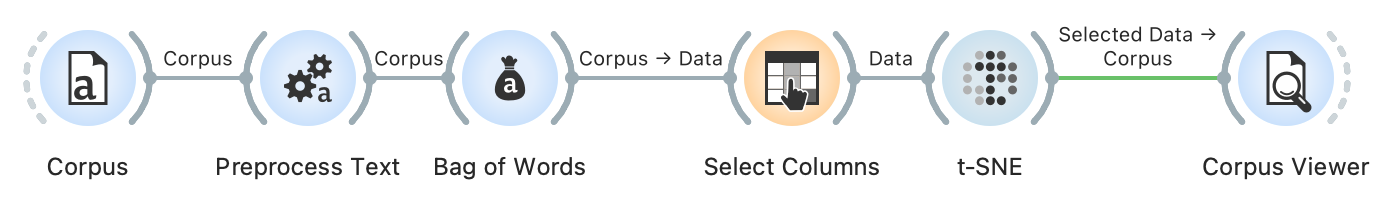
\includegraphics[width=\linewidth]{workflow.png}%
  \caption{$\;$}
\end{figure*}
\vspace{-0.3cm}

First, we need to preprocess the data with \widget{Preprocess Text}. We will use a special Tweet tokenizer, that was pre-trained on millions of tweets. This will retain special words, such as @mentions, \#hashtags, and emojis :). As the Tweet tokenizer doesn't remove punctuation, we will remove it with the pre-set Regexp filter.

This time we have a lot of unique tokens and things might get painfully slow. To narrow down the tokens even further, we can filter out all the infrequent words with \emph{Document frequency}. Set the lower threshold to 0.01 - this means we will omit all the words appearing in less than 1\% of the tweets.

\begin{figure*}[h]
    \centering
    \infinitewidthbox{
      \stackinset{r}{-0.4\linewidth}{t}{+0.15\linewidth}
      {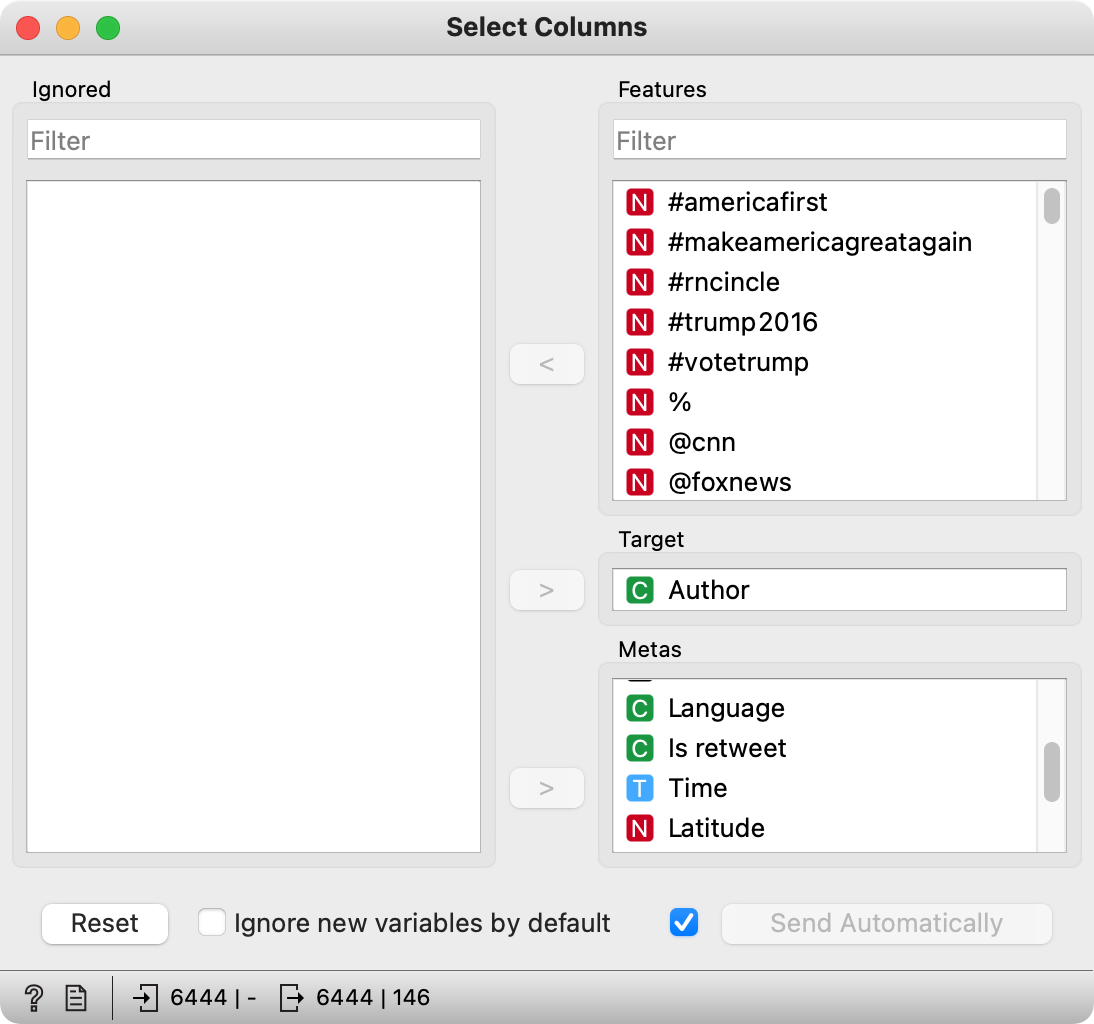
\includegraphics[scale=0.45]{select-columns.png}}
      {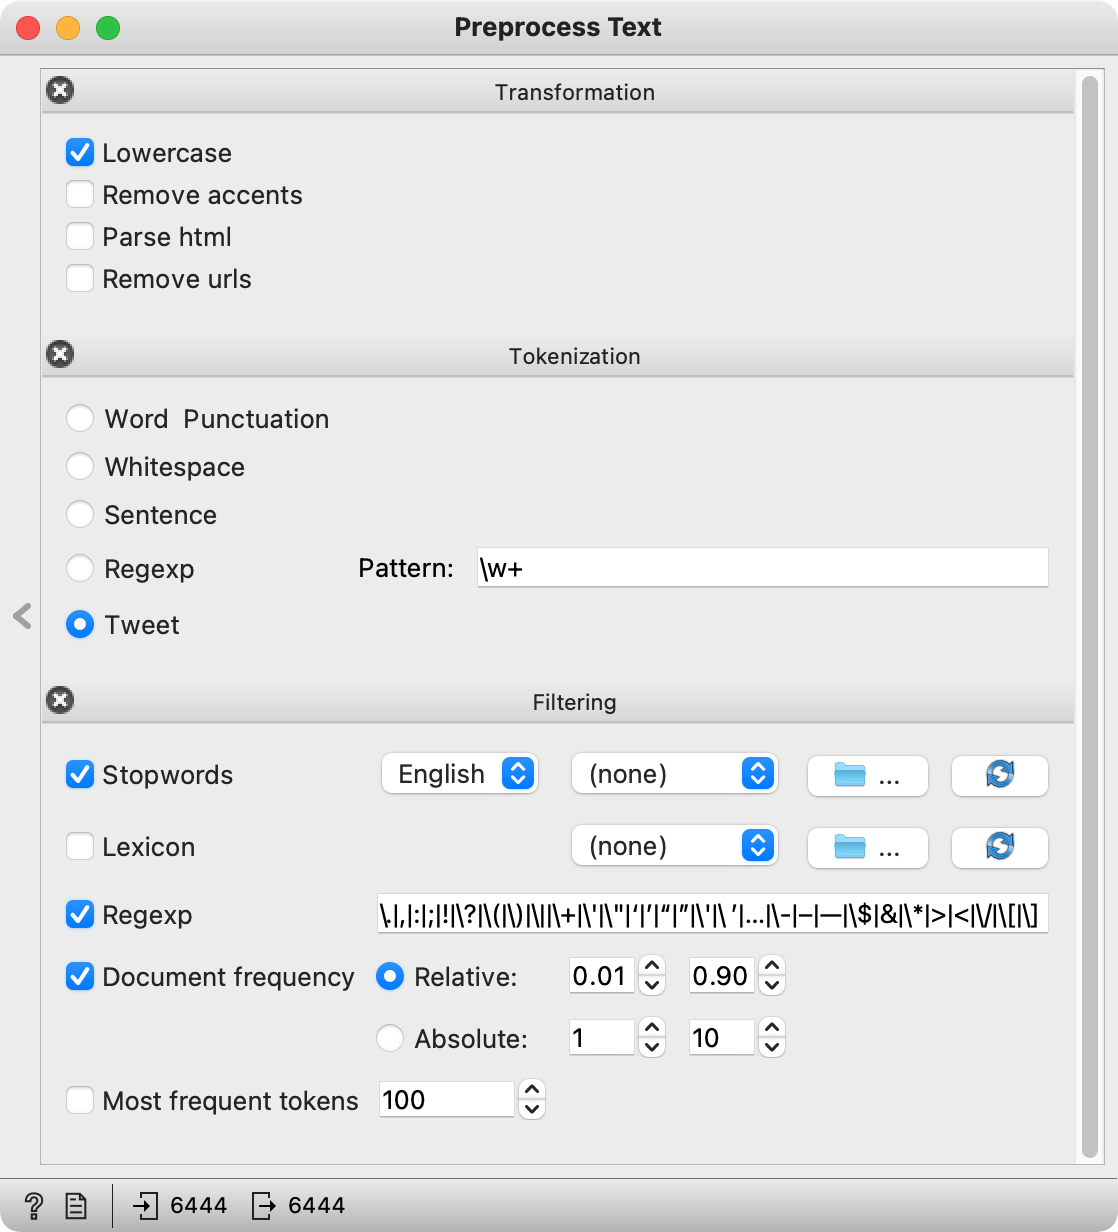
\includegraphics[scale=0.45]{preprocessing.png}}
      \hspace{6cm}
      }
    \caption{$\;$}
\end{figure*}

Great, now we are left with manageable 146 tokens. Pass the preprocessed data to \widget{Bag of Words}. If we check the results of BoW in a \widget{Data Table}, we can see there are some features we don't wish to consider in the analysis. To remove them from the analysis, use \widget{Select Columns} and put all those non-textual features to meta attributes.

Next, we will use t-SNE, a special dimensionality reduction technique that allows us to observe the data in a 2D plane. In this visualization, data instances that are similar to each other, will be put closer together. This usually results in distinct clusters, just like in our example.

\vspace{-0.2cm}
\begin{figure*}[h]
  \centering
  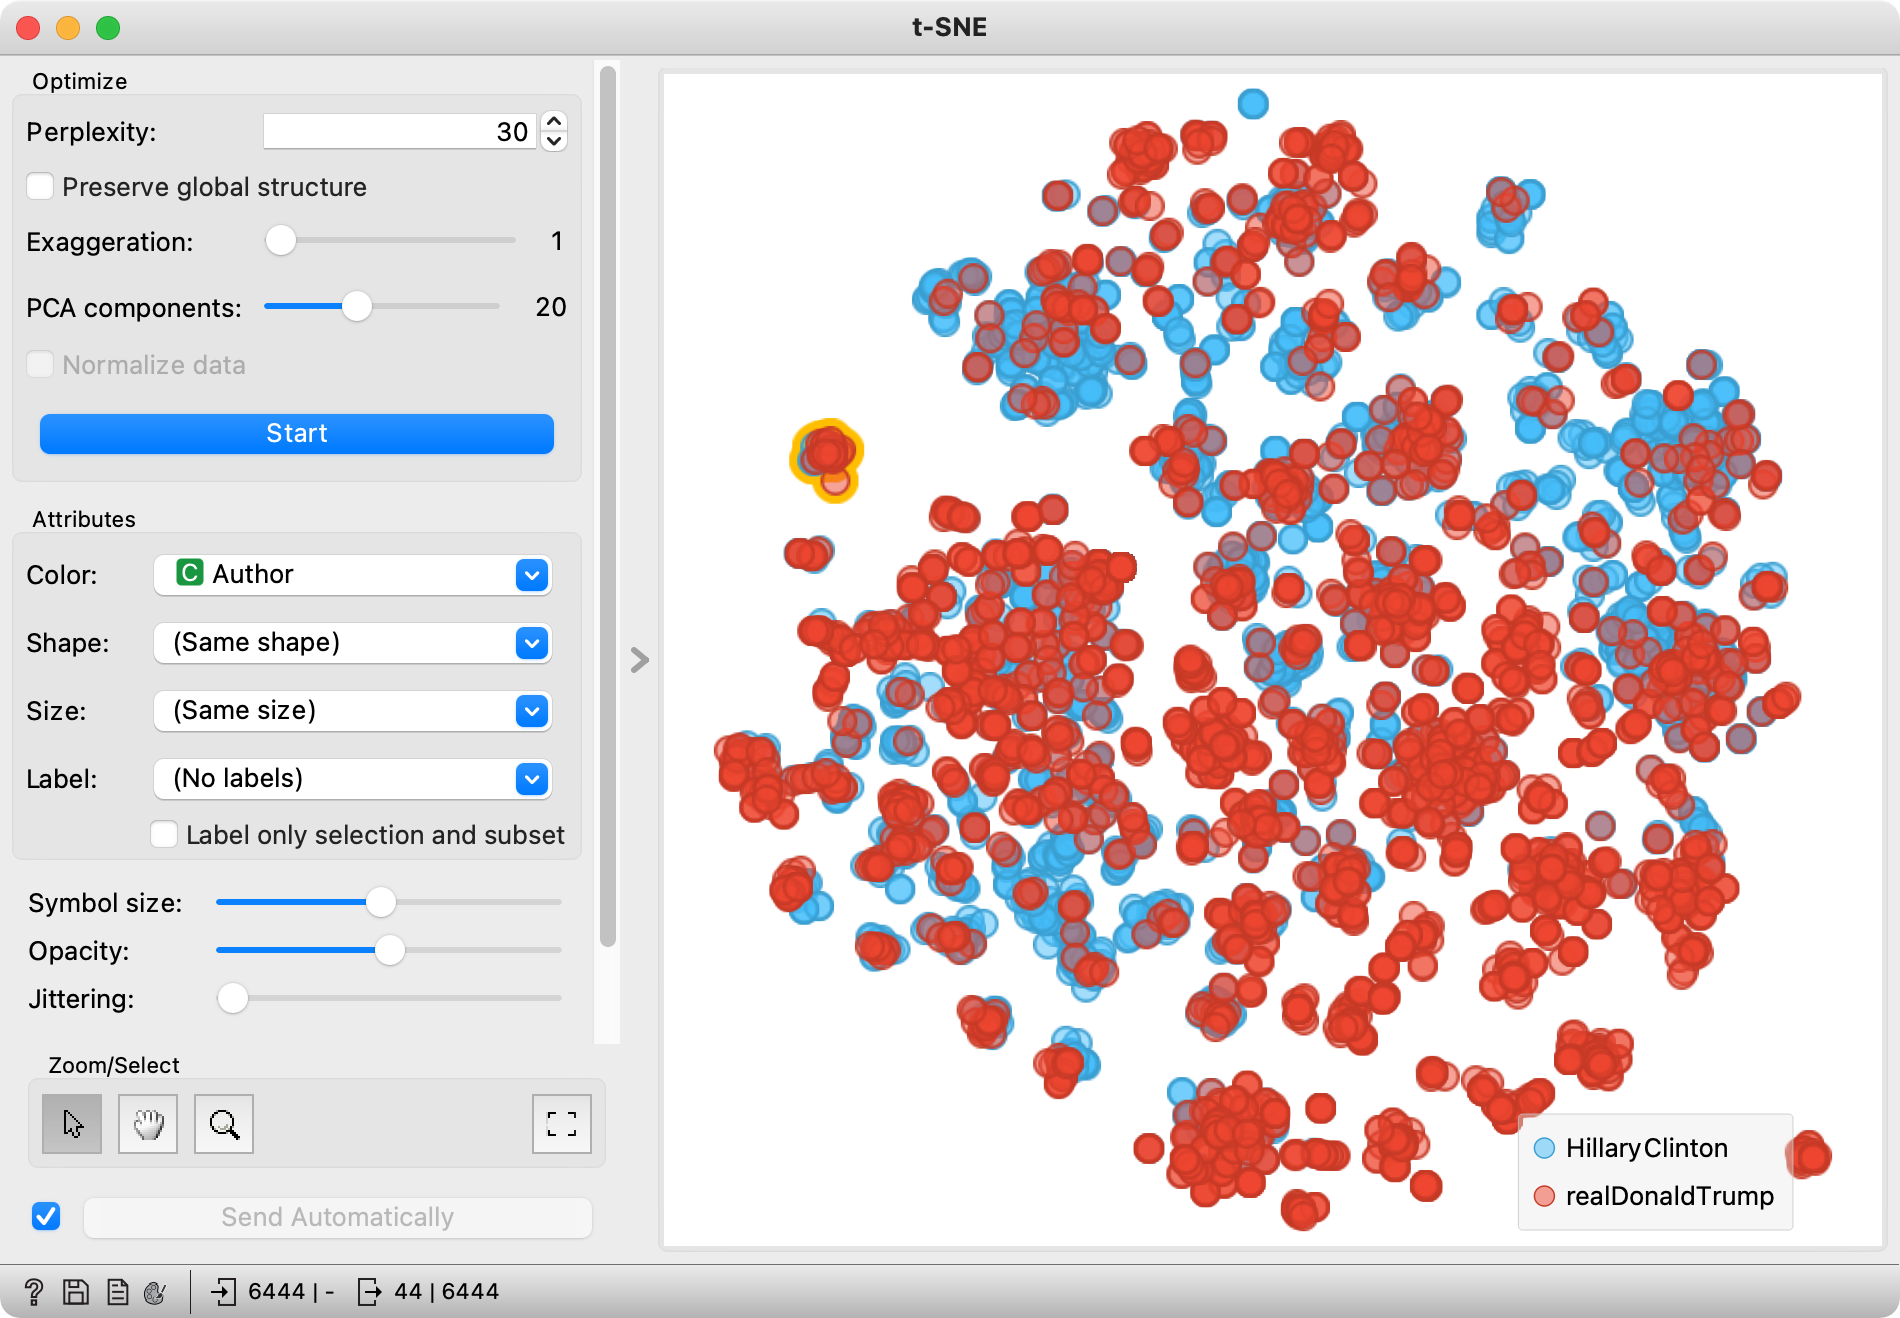
\includegraphics[width=0.8\linewidth]{t-sne.png}%
  \caption{$\;$}
\end{figure*}
\vspace{-0.3cm}

Select a cluster and inspect it in a \widget{Corpus Viewer}. What are the documents about? Does the cluster make sense?

\vspace{-0.2cm}
\begin{figure}[h]
  \centering
  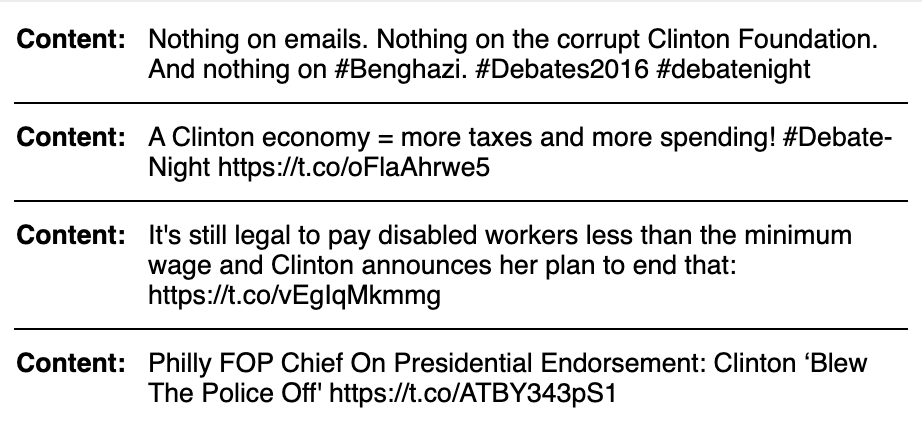
\includegraphics[width=\linewidth]{corpus-viewer.png}%
  \caption{$\;$}
\end{figure}
\vspace{-0.3cm}
